\documentclass{standalone}
\usepackage{amsmath}
\usepackage{tikz}
\usepackage{rotating}
\usetikzlibrary{shapes.geometric, arrows}

\tikzstyle{startstop} = [rectangle, rounded corners, 
minimum width=3cm, 
minimum height=1cm,
text centered, 
draw=black, 
fill=red!30]

\tikzstyle{io} = [trapezium, 
trapezium stretches=true, % A later addition
trapezium left angle=70, 
trapezium right angle=110, 
minimum width=3cm, 
minimum height=1cm, text centered, 
draw=black, fill=blue!30]

\tikzstyle{process} = [rectangle, 
minimum width=3cm, 
minimum height=1cm, 
text centered,  
draw=black, 
fill=orange!30]

\tikzstyle{decision} = [diamond, 
minimum width=3cm, 
minimum height=1cm, 
text centered, 
draw=black, 
fill=green!30]
\tikzstyle{arrow} = [thick,->,>=stealth]
\begin{document}

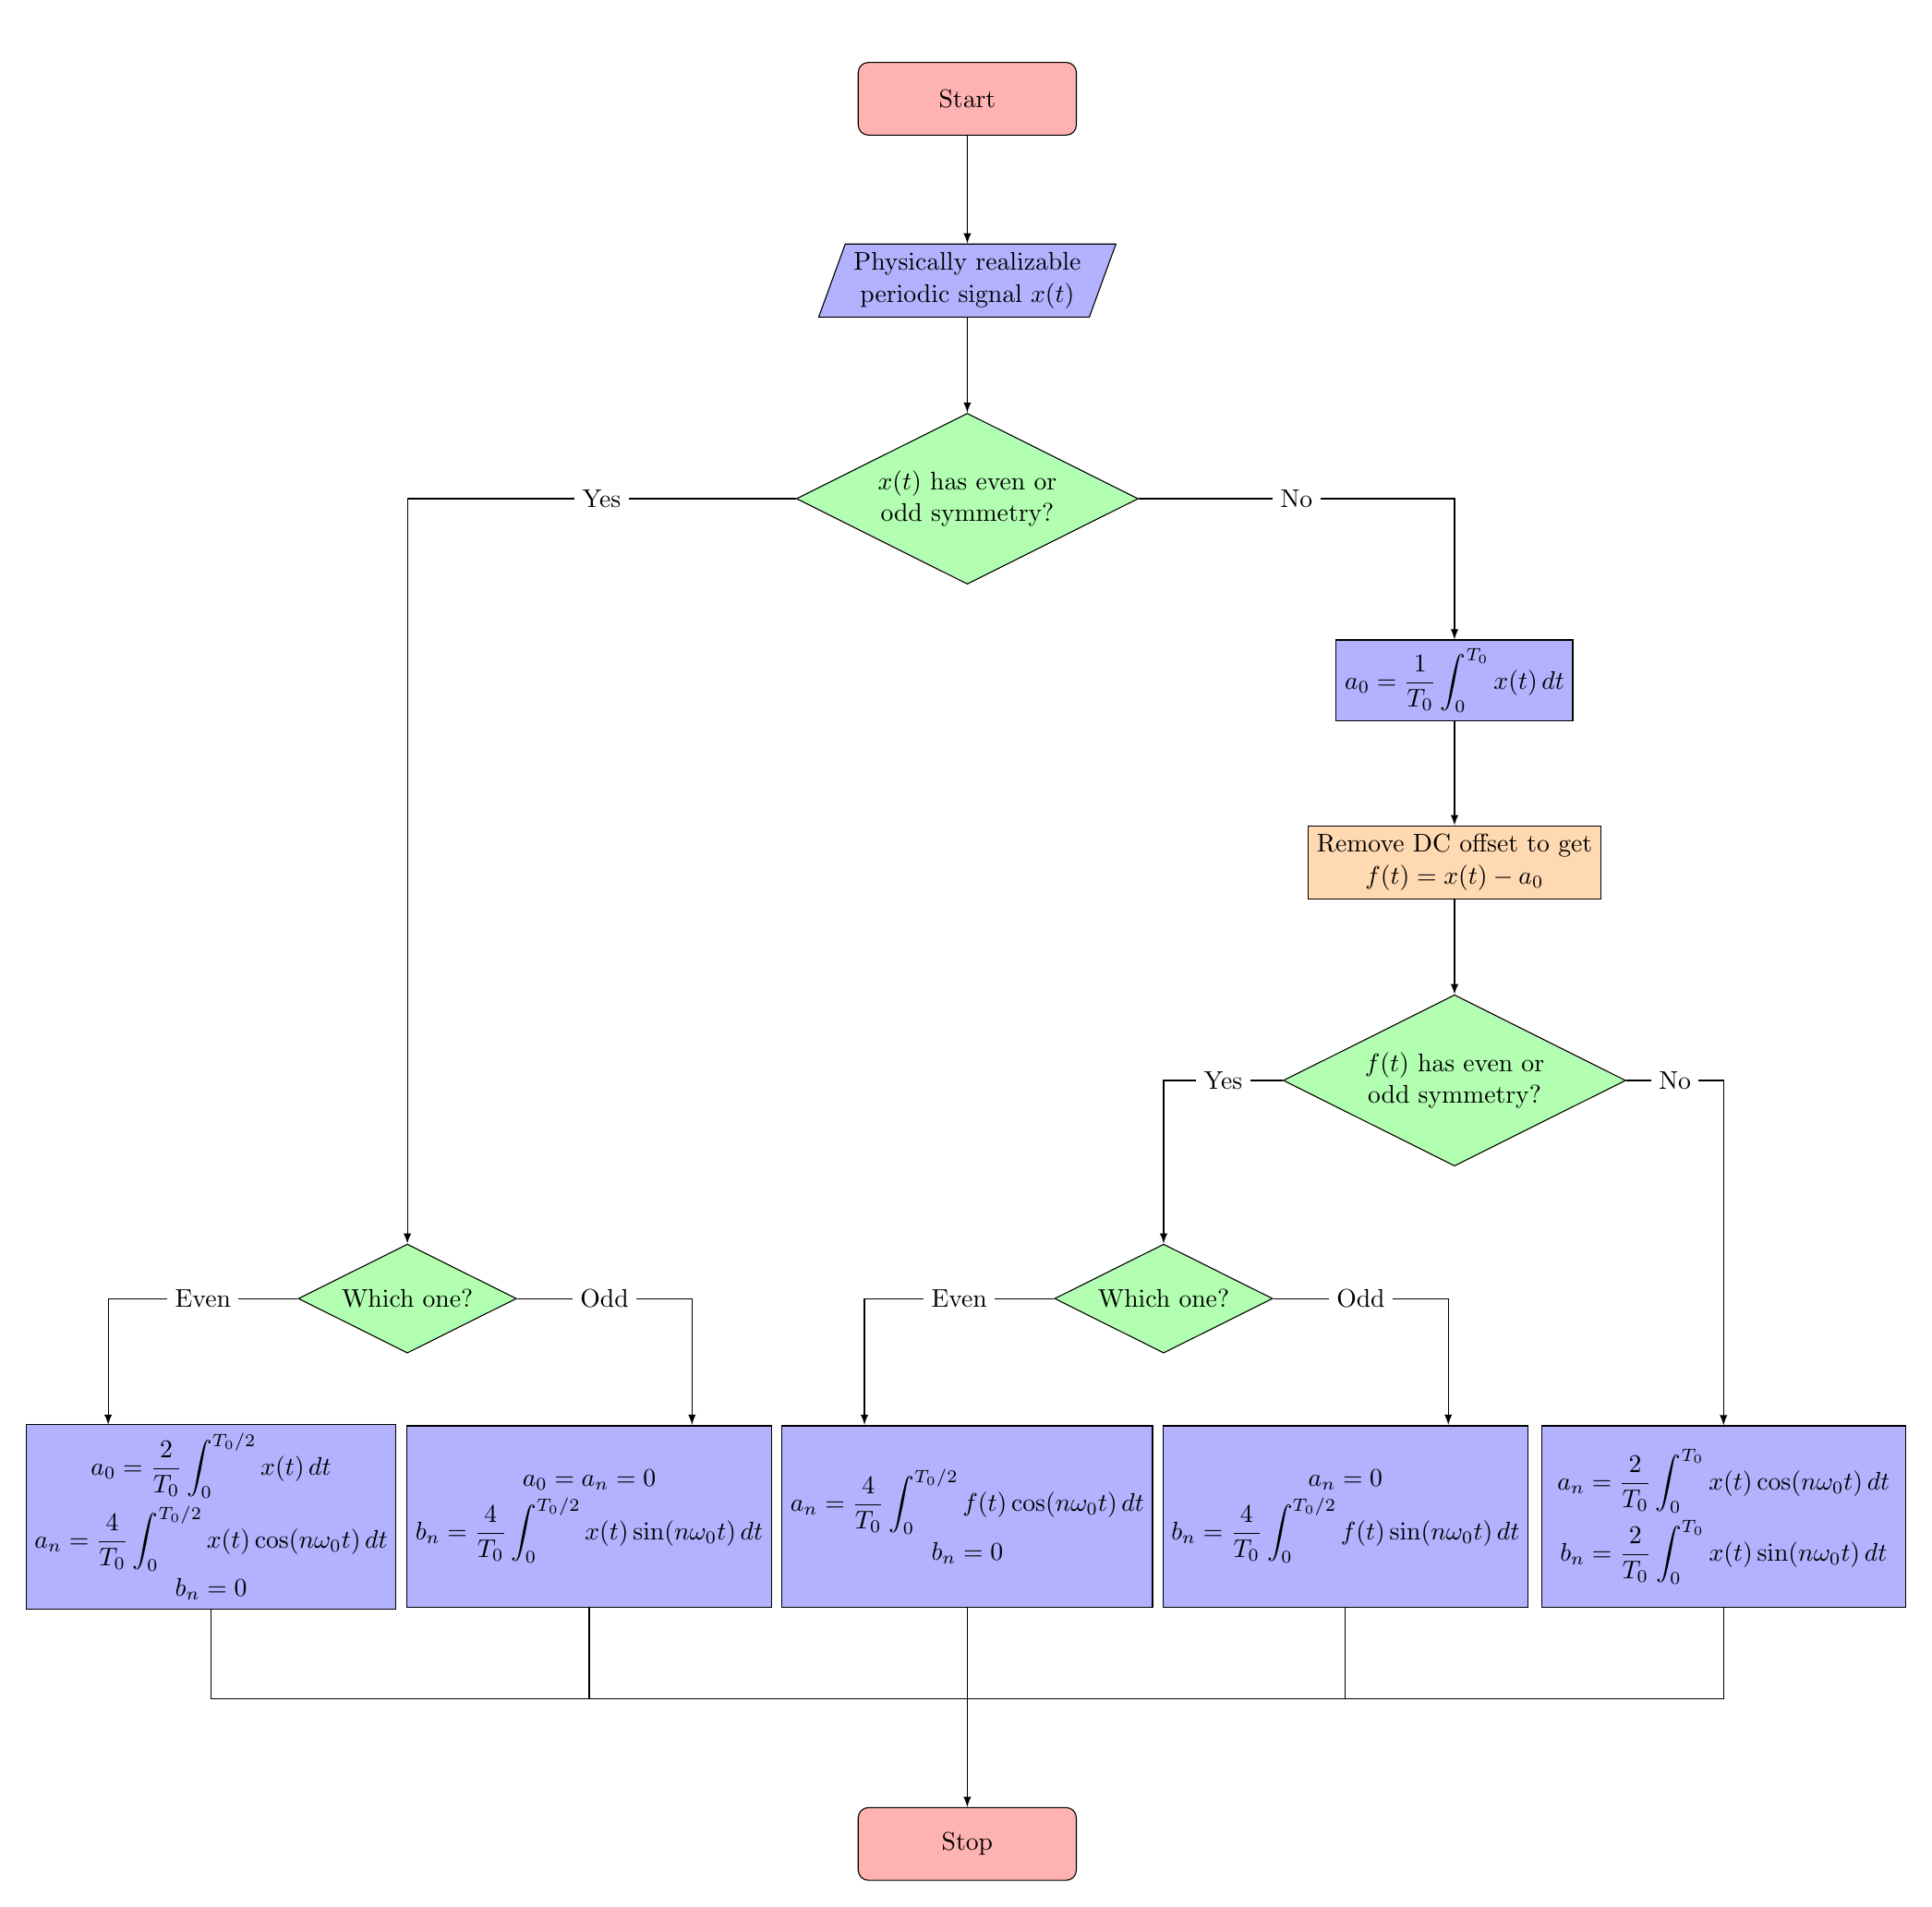
\begin{tikzpicture}[node distance=2cm]

\node (stop) [startstop] {Stop};
\node[coordinate,above of=stop] (connect) {};
\node (pro5c) [process, above of=stop, yshift=2.5cm, minimum width=5cm, minimum height=2.5cm, fill=blue!30] {\shortstack{$a_n = \dfrac{4}{T_0}\displaystyle\int_{0}^{T_0/2}f(t)\cos(n\omega_0 t)\,dt$ \\ $b_n = 0$}};
\node (pro5d) [process, right of=pro5c, xshift=3.2cm, minimum width=5cm, minimum height=2.5cm, fill=blue!30] {\shortstack{$a_n = 0$ \\ $b_n = \dfrac{4}{T_0}\displaystyle\int_{0}^{T_0/2}f(t)\sin(n\omega_0 t)\,dt$}};
\node (pro5e) [process, right of=pro5d, xshift=3.2cm, minimum width=5cm, minimum height=2.5cm, fill=blue!30] {\shortstack{$a_n = \dfrac{2}{T_0}\displaystyle\int_{0}^{T_0}x(t)\cos(n\omega_0 t)\,dt$ \\ $b_n = \dfrac{2}{T_0}\displaystyle\int_{0}^{T_0}x(t)\sin(n\omega_0 t)\,dt$}};
\node (pro5b) [process, left of=pro5c, xshift=-3.2cm, minimum width=5cm, minimum height=2.5cm, fill=blue!30] {\shortstack{$a_0 = a_n = 0$ \\ $b_n = \dfrac{4}{T_0}\displaystyle\int_{0}^{T_0/2}x(t)\sin(n\omega_0 t)\,dt$ }};
\node (pro5a) [process, left of=pro5b, xshift=-3.2cm, minimum width=5cm, minimum height=2.5cm, fill=blue!30] {\shortstack{$a_0 = \dfrac{2}{T_0}\displaystyle\int_{0}^{T_0/2}x(t)\,dt$ \\ $a_n = \dfrac{4}{T_0}\displaystyle\int_{0}^{T_0/2}x(t)\cos(n\omega_0 t)\,dt$ \\ $b_n = 0$}};
\draw[-] (pro5a) |- (connect);
\draw[-] (pro5b) |- (connect);
\draw[-] (pro5c) edge (connect);
\draw[-] (pro5d) |- (connect);
\draw[-] (pro5e) |- (connect);
\draw[-latex] (connect) -- (stop);

\node (dec4a) [decision, above of=pro5a, xshift=2.7cm, yshift=1cm, aspect=2] {Which one?};
\node[coordinate, above left of=pro5a, yshift=-0.15cm] (even4a) {};
\node[coordinate, above right of=pro5b, yshift=-0.15cm] (odd4a) {};
\draw[-latex] (dec4a) -| (even4a) node[pos=0.25,fill=white,inner sep=3pt]{Even};
\draw[-latex] (dec4a) -| (odd4a) node[pos=0.25,fill=white,inner sep=3pt]{Odd};
\node (dec4b) [decision, above of=pro5c, xshift=2.7cm, yshift=1cm, aspect=2] {Which one?};
\node[coordinate, above left of=pro5c, yshift=-0.15cm] (even4b) {};
\node[coordinate, above right of=pro5d, yshift=-0.15cm] (odd4b) {};
\draw[-latex] (dec4b) -| (even4b) node[pos=0.25,fill=white,inner sep=3pt]{Even};
\draw[-latex] (dec4b) -| (odd4b) node[pos=0.25,fill=white,inner sep=3pt]{Odd};

\node (dec3) [decision, above of=dec4b, xshift=4cm, yshift=1cm, aspect=2] {\shortstack{$f(t)$ has even or \\ odd symmetry?}};
\draw[-latex] (dec3) -| (dec4b) node[pos=0.25,fill=white,inner sep=3pt]{Yes};
\draw[-latex] (dec3) -| (pro5e) node[pos=0.25,fill=white,inner sep=3pt]{No};
\node (pro3) [process, above of=dec3, yshift=1cm] {\shortstack{Remove DC offset to get \\ $f(t) = x(t) - a_0$}};
\node (pro2) [process, above of=pro3, yshift=0.5cm, fill=blue!30] {$a_0 = \dfrac{1}{T_0}\displaystyle\int_{0}^{T_0}x(t)\,dt$};
\draw[-latex] (pro2) edge (pro3);
\draw[-latex] (pro3) edge (dec3);

\node (dec1) [decision, above of=pro5c, yshift=12cm, aspect=2] {\shortstack{$x(t)$ has even or \\ odd symmetry?}};
\draw[-latex] (dec1) -| (dec4a) node[pos=0.25,fill=white,inner sep=3pt]{Yes};
\draw[-latex] (dec1) -| (pro2) node[pos=0.25,fill=white,inner sep=3pt]{No};

\node (in1) [io, above of=dec1, yshift=1cm] {\shortstack{Physically realizable \\ periodic signal $x(t)$}};
\node (start) [startstop, above of=in1, yshift=0.5cm] {Start};
\draw[-latex] (start) edge (in1);
\draw[-latex] (in1) edge (dec1);
\node[coordinate,above of=start, yshift=-1cm] (blank) {};
\draw[-] (blank) -| (blank);

\end{tikzpicture}
\end{document}